\section{Budgeted Evidence Selection}
\label{sec:selector}

Let $\Tset(I)=\{t_i\}_{i=1}^{N_I}$ be the tiles from source image $I$.
The detector produces confidence $c_i\in[0,1]$ and predicted count $n_i$.
The evidence score is
\begin{equation}
q_i=c_i+\frac{\min(n_i,20)}{20}.
\label{eq:score}
\end{equation}
The cap prevents a single unusually dense tile from dominating the ranking.
For budget $K$ and exploration ratio $\rho$, we set
\begin{equation}
K_{\mathrm{explore}}=\operatorname{round}(\rho K),\qquad
K_{\mathrm{exploit}}=K-K_{\mathrm{explore}}.
\label{eq:allocation}
\end{equation}
The selected set is
\begin{equation}
\Eset_K(I)=
\operatorname{TopK}_{K_{\mathrm{exploit}}}(q_i)
\cup
\operatorname{Explore}_{K_{\mathrm{explore}}}
(\Tset(I)\setminus\Eset_{\mathrm{exploit}}).
\label{eq:selector}
\end{equation}
The default $K=8$, $\rho=0.25$ therefore uses six exploitative and two
exploratory tiles.  All VLMs receive exactly the same selected images and task
schema for a given source.

\paragraph{Validation metrics.}
For source objects $\mathcal{B}_I$, evidence recall at threshold $\eta=0.5$ is
\begin{equation}
R_{\mathrm{ev}}(I)=\frac{1}{|\mathcal{B}_I|}
\sum_{b\in\mathcal{B}_I}
\mathbf{1}\!\left[\max_{t\in\Eset_K(I)}v(b,t)\geq\eta\right].
\label{eq:evidence-recall}
\end{equation}
Spatial coverage is the union area of selected tiles divided by source area.
Overlap redundancy is
\begin{equation}
D_{\mathrm{ov}}(I)=
\frac{\sum_{t\in\Eset_K(I)}\operatorname{area}(t)}
{\operatorname{area}(\cup_{t\in\Eset_K(I)}t)}-1.
\label{eq:redundancy}
\end{equation}
We additionally report boundary-truncation rate and the fraction of prepared
hard-negative tiles retained by a selector.  Confidence intervals use 1,000
source-level bootstrap resamples.  Randomized selectors use ten repetitions.
\Cref{tab:selector-b8} reports the matched $K=8$ comparison.

\begin{table*}[t]
\centering
\caption{Validation-only selector audit at $K=8$.  Values are source means;
parentheses give source-bootstrap 95\% confidence intervals.  Oracle and
shuffled-score controls are omitted because they are diagnostics, not
deployable selectors.}
\label{tab:selector-b8}
\small
\setlength{\tabcolsep}{4.5pt}
\begin{tabular}{lccccc}
\toprule
Selector & Evidence recall & Spatial coverage & Redundancy & Boundary trunc. & Hard-neg. recall \\
\midrule
Random & .352 (.335--.382) & .361 (.359--.364) & .141 (.136--.146) & .459 (.423--.492) & .231 (.209--.253) \\
Spatial uniform & .438 (.415--.464) & .411 (.409--.413) & .000 (.000--.000) & .401 (.371--.431) & .196 (.136--.257) \\
Confidence top-$K$ & .384 (.350--.425) & .340 (.334--.346) & .214 (.194--.234) & .495 (.449--.538) & .024 (.000--.065) \\
Count top-$K$ & \textbf{.455} (.420--.496) & .330 (.324--.337) & .252 (.226--.282) & \textbf{.398} (.359--.437) & .015 (.000--.043) \\
Combined top-$K$ & .451 (.416--.494) & .330 (.324--.336) & .254 (.229--.285) & .474 (.424--.516) & .007 (.000--.018) \\
Exploit--explore & .439 (.410--.474) & .345 (.341--.349) & .196 (.183--.212) & .486 (.438--.529) & .067 (.050--.085) \\
\bottomrule
\end{tabular}
\end{table*}

The audit exposes a genuine trade-off rather than a uniformly dominant method.
Count top-$K$ yields the highest validation evidence recall at $K=8$.
Exploit--explore reduces overlap redundancy by 22.7\% relative to combined
top-$K$ and raises hard-negative retention from 0.7\% to 6.7\%, but its evidence
recall is lower by 1.2 points.  The operating point must therefore match the
downstream reliability objective rather than maximize one metric alone.

\begin{figure*}[t]
\centering
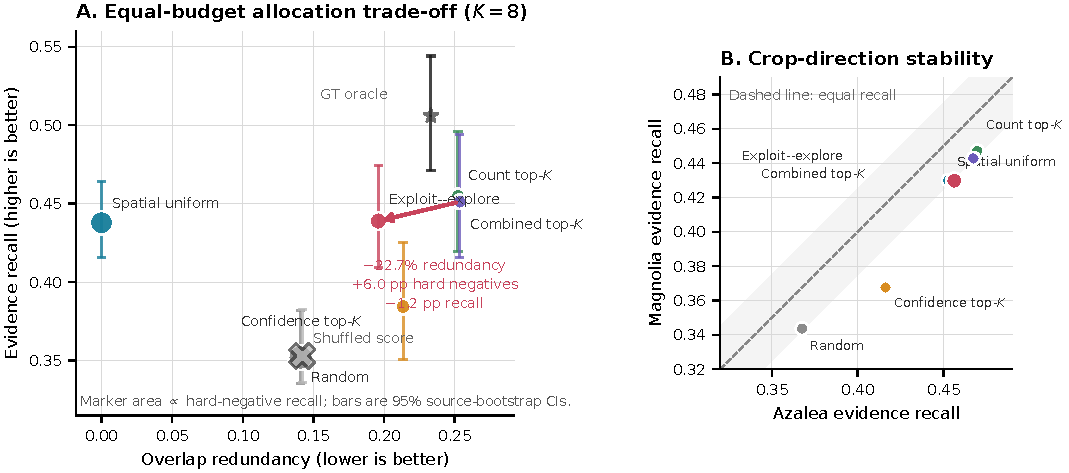
\includegraphics[width=.98\textwidth]{figures/selector_tradeoff_map.pdf}
\caption{Mechanism-level selector audit at the matched budget $K=8$.
\textbf{A:} Evidence recall versus overlap redundancy; vertical bars are 95\%
source-bootstrap intervals and marker area is proportional to hard-negative
recall.  Stars denote non-deployable diagnostics.  The arrow isolates the
combined-to-exploit--explore change.  \textbf{B:} Crop-specific evidence recall;
distance from the equality line reveals directional sensitivity that a pooled
mean would hide.}
\label{fig:selector-tradeoff}
\end{figure*}

\Cref{fig:selector-tradeoff} exposes the equal-budget trade-off and crop
direction, while \cref{fig:selector-sweep} tests whether it persists across the
complete budget range.

\begin{figure*}[t]
\centering
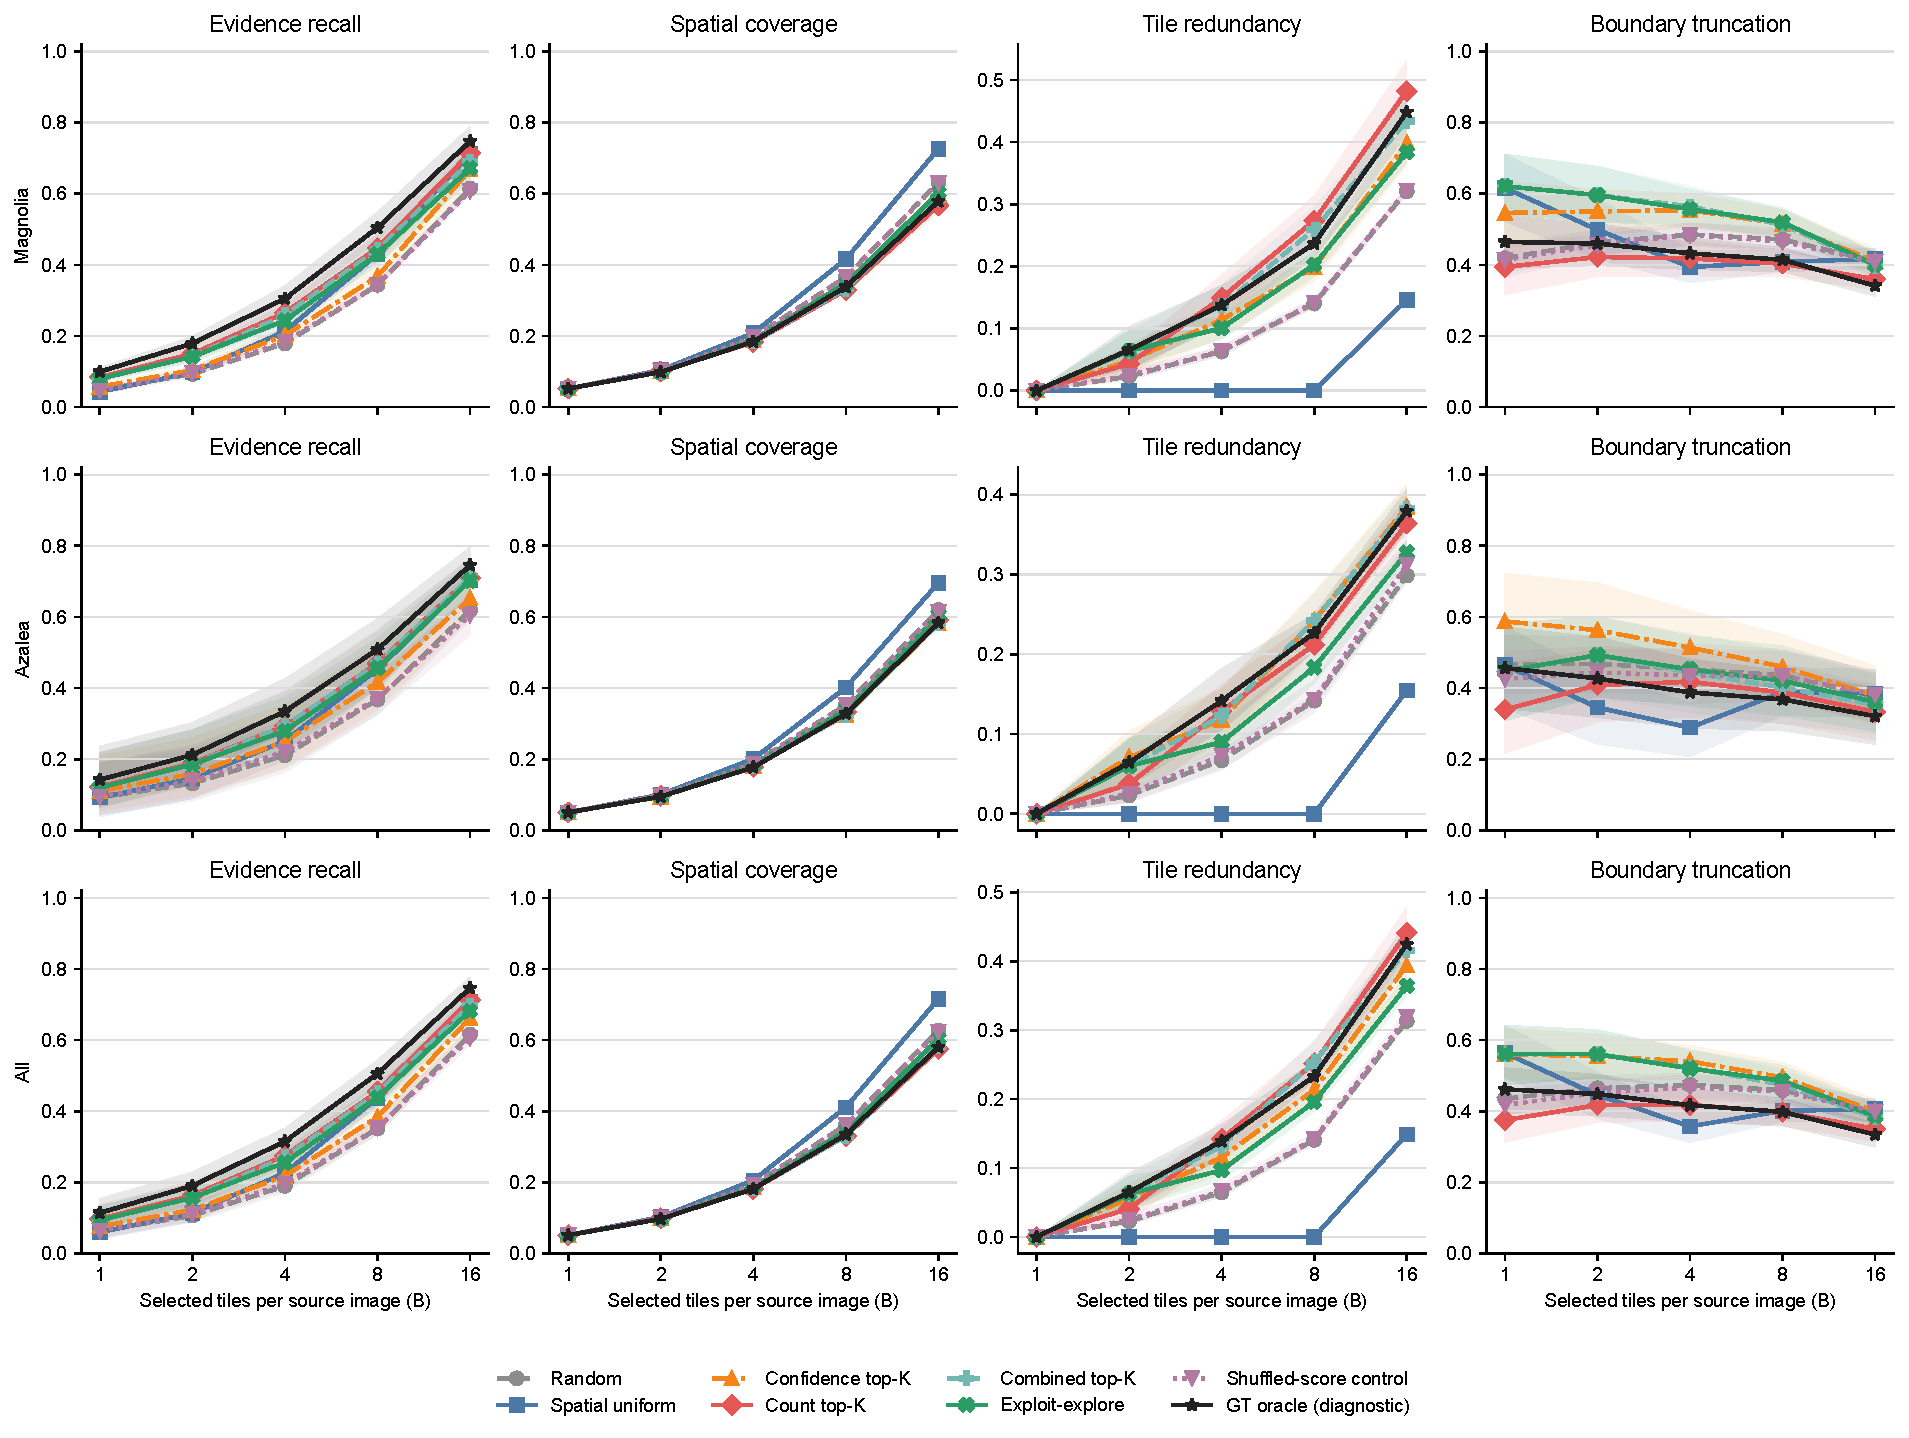
\includegraphics[width=.98\textwidth]{figures/selector_budget_audit.pdf}
\caption{Complete validation-only budget sweep.  Curves show source-level
means and 95\% source-bootstrap intervals across both crop domains and their
pooled source set.}
\label{fig:selector-sweep}
\end{figure*}
